\subsection{Алгоритмы машинного обучения}

Классические алгоритмы машинного обучения (МО) широко применяются для обнаружения аномалий в контейнерных средах благодаря способности выявлять скрытые закономерности в данных и определять отклонения от типичного поведения системы. В отличие от статических методов, такие алгоритмы опираются не на заранее заданные правила, а на статистические свойства обучающей выборки и особенности распределения наблюдений \cite{AD_Survey}.

Для анализа контейнерных сред и Kubernetes-кластеров классические алгоритмы МО могут применяться к различным типам данных: audit-логам, метрикам использования ресурсов, сетевой телеметрии, событиям взаимодействия между подами и признакам поведения пользователей или сервисных аккаунтов.

К числу наиболее распространённых алгоритмов машинного обучения, применяемых для обнаружения аномалий, относятся:

\begin{itemize}
    \item \textbf{K-ближайших соседей (K-Nearest Neighbors, K-NN)} — метод, основанный на оценке близости объекта к другим наблюдениям в пространстве признаков \cite{knn};
    \item \textbf{Isolation Forest (iForest)} — алгоритм, основанный на случайной изоляции объектов с помощью ансамбля деревьев \cite{iForest};
    \item \textbf{Random Cut Forest (RCF)} — метод, использующий ансамбль случайных разрезов пространства признаков и подходящий для потоковых данных \cite{RCF}.
\end{itemize}

\subsubsection{Метод K-ближайших соседей}

\textbf{K-NN} — алгоритм классификации и регрессии, основанный на гипотезе компактности, которая предполагает, что расположенные близко друг к другу объекты в пространстве признаков имеют схожие значения целевой переменной или принадлежат к одному классу \cite{knn}.

Принцип работы заключается в том, что для каждого нового наблюдения x алгоритм ищет k ближайших «соседей» в обучающей выборке и на основе расстояния/плотности соседей принимает решение (классификация) или вычисляет степень аномальности (anomaly score). Существуют несколько метрик расстояний:

\begin{itemize}
    \item Евклидово расстояние: \( d(\mathbf{x},\mathbf{y}) = \sqrt{\sum_{i=1}^n (x_i - y_i)^2} \);
    \item Манхэттен (L1) расстояние: \( d(\mathbf{x},\mathbf{y}) = \sum_{i=1}^n |x_i - y_i| \);
    \item Метрика Чебышева: \( d(\mathbf{x},\mathbf{y}) = \max_{i=1,\dots,n} |x_i - y_i| \).
\end{itemize}

Преимущества:

\begin{itemize}
    \item простота реализации: алгоритм легко адаптируется к разным типам данных;
    \item гибкость: может использоваться для задач классификации, регрессии и выявления аномалий;
\end{itemize}

Ограничения:

\begin{itemize}
    \item при большом объёме данных и высоком количестве признаков вычисление расстояний до всех соседей может быть ресурсоёмким;
    \item работает только с чиловыми признаками, поэтому необходима предобработка для данных. 
\end{itemize}

\subsubsection{Алгоритм Isolation Forest}

\textbf{Алгоритм Isolation Forest (iForest)} — метод обнаружения аномалий, основанный на идее изоляции объектов путём построения ансамбля случайных бинарных деревьев. Его фундаментальная концепция заключается в том, что образцы, которые проникают глубже в дерево, с меньшей вероятностью будут аномалиями, поскольку для их изоляции требуется больше разрезов, а образцы, которые оказываются в более коротких ветвях, указывают на аномалии, поскольку дереву проще отделить их от других наблюдений\cite{iForest}. 

На рисунке~\ref{fig:IF_png} показана концепция обнаружения аномалий с помощью Isolation Forest.

\begin{figure}
    \centering
    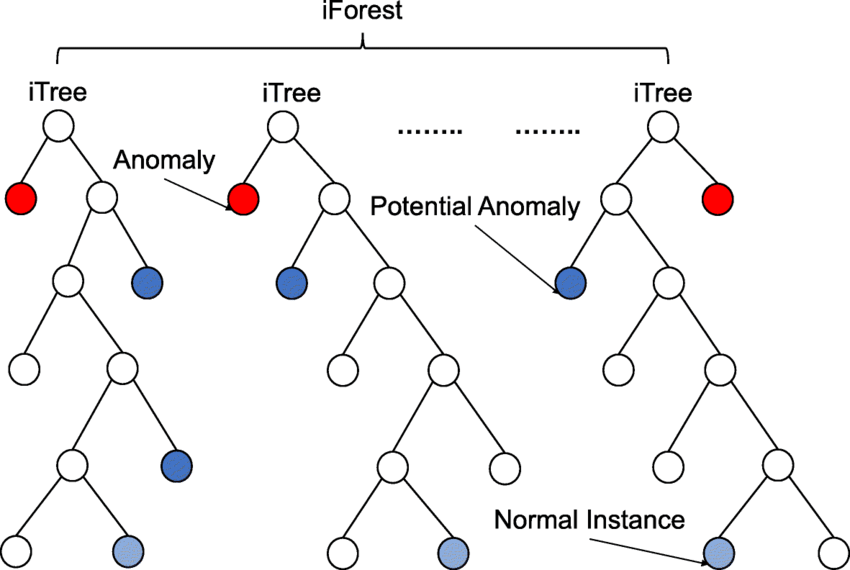
\includegraphics[scale=0.3]{inc/images/Isolation-Forest-learned}
    \caption{Схема выявления аномалий на основе Isolation Forest \cite{IF_png}.}
    \label{fig:IF_png}
\end{figure}

Принцип работы алгоритма заключается в следующем. Из исходного множества данных формируется ансамбль деревьев iTree \(t\), каждое из которых строится на случайно выбранной подвыборке данных размера \(\psi\). При построении дерева на каждом узле случайно выбирается признак \(q\) и случайный порог \(p\) из интервала \([\min_{x\in X} x_q,\;\max_{x\in X} x_q]\); затем пространство рекурсивно делится по этому порогу.

Построение iTree происходит следующем образом:

\begin{itemize}
    \item Выбирается подвыборка размера \(\psi\).
    \item Рекурсивно: пока \( |X|>1 \) и глубина ($height$) $<$ $height\_limit$:
    \begin{itemize}
        \item случайно выбрать признак \(q\) из множества признаков;
        \item случайно выбрать порог \(p\) из интервала $[\min_q,\;\max_q]$;
        \item разделить точки на множества $\{x\in X \mid x_q < p\}$ и $\{x\in X \mid x_q \ge p\}$ и рекурсивно строить дочерние узлы.
    \end{itemize}
    \item Остановить, если $|X|=1$ либо достигнут предельный уровень (height limit).
\end{itemize}

Для оценки аномальности объекта сначала вычисляют среднюю длину пути по всем деревьям ансамбля, \(E(h(x))\), приведенную в формуле~\ref{E_h}. 

\begin{equation}\label{E_h}
    E(h(x)) \;=\; \frac{1}{t}\sum_{i=1}^{t} h_i(x)
\end{equation}

где \(t\) — число деревьев.

Далее вычисляют нормирующую функцию \(c(n)\), используемую для приведения средней длины пути к масштабу, независимому от размера выборки \(n\), вычисляемую по формуле ~\ref{c_n}.

\begin{equation}\label{c_n}
    c(n) \;=\; 2H_{\,n-1} \;-\; \frac{2(n-1)}{n}
\end{equation}

где $H_{n}$ - гармоническое число

Наконец, для получения численной оценки аномальности применяют нормализацию средней длины пути \(E(h(x))\) по значению функции \(c(n)\); окончательная формула для вычисление значения аномальности приведена в ~\ref{s_x_n}.

\begin{equation}\label{s_x_n}
    s(x, n) \;=\; 2^{-\frac{E(h(x))}{c(n)}}
\end{equation}

Значение \(s(x,n)\), близкое к 1, указывает на высокую степень аномальности.

\subsubsection{Алгоритм Random Cut Forest}

\textbf{Алгоритм Random Cut Forest (RCF)} — это метод обнаружения аномалий, основанный на построении ансамбля случайных деревьев разрезов. В отличие от Isolation Forest, который изолирует точки с помощью последовательных случайных бинарных разбиений подвыборок, RCF формирует деревья непосредственно на основе случайных геометрических разрезов пространства признаков, что позволяет корректно обновлять и поддерживать модель при потоковом поступлении данных \cite{RCF}.

Основная идея заключается в том, что аномальные точки — это такие объекты, добавление или удаление которых вызывает значительное изменение геометрической структуры дерева, то есть существенно изменяет распределение разрезов, формирующих дерево. Алгоритм использует понятие размера проекции (displacement) и сопоставимой дисперсии (co-displacement), которые измеряют, насколько сильно добавление или удаление точки влияет на «геометрическую плотность» соседних точек в пространстве.

Алгоритм построения деревьев в RCF схож с алгоритмом iForest, за исключением того, как выбирается признак \(q\): вероятность выбора \(q\) пропорциональна длине стороны данного признака. Пусть имеется множество точек \(S = \{x_1, x_2, \dots, x_n\} \subset R^d\). Далее рекурсивно строится дерево \(T(S)\):
\begin{enumerate}
    \item Высчитываются длины сторон гиперпрямоугольника по формуле ~\ref{l_i}.

\begin{equation}\label{l_i}
    l_i \;=\; \max_{x \in S} x_i - \min_{x \in S} x_i
\end{equation}

    \item Строится гиперпрямоугольник (bounding box) $$B(S) = [\min_{x \in S} x_1, \max_{x \in S} x_1] \times  \dots \times [\min_{x \in S} x_d, \max_{x \in S} x_d],$$ охватывающий все точки множества \(S\).
    \item Вероятность выбора признака \(q \in Q\) высчитывается по формуле ~\ref{P_q}.  

\begin{equation}\label{P_q}
    P(q) \;=\; \frac{l_q}{\sum_{i \in Q} l_i}
\end{equation}

    \item Выбирается порог \(p\), равномерно выбранный из интервала \([\min_{x \in S} x_q, \max_{x \in S} x_q]\).
    \item Разрезом \((q,p)\) пространство \(B(S)\) разделяется на две части: $$S_L = \{ x\in S \mid x_q < p \}$$ и $$S_R = \{ x\in S \mid x_q \ge p \}$$
\end{enumerate}

В отличие от Isolation Forest, RCF не ограничивается метрикой глубины узла, а оценивает влияние объекта на геометрическую структуру данных. Это делает метод более устойчивым к изменениям плотности и эффективным для потоковых сценариев, где требуется онлайн-обновление модели без полной перестройки.